\renewcommand{\thechapter}{C}
\chapter{Appendix for Chapter~\ref{chap:ch3}}\label{APP:C}
% \phantomsection\addcontentsline{toc}{chapter}{Appendices}

\renewcommand{\thesection}{C.\arabic{section}}
\renewcommand{\thesubsection}{C.\arabic{section}.\arabic{subsection}}
\renewcommand{\thefigure}{C.\arabic{figure}}
\renewcommand{\thetable}{C.\arabic{table}}
\renewcommand{\theequation}{C.\arabic{equation}}

\section{Theoretical Proofs and Discussions}
% \stoptoc
%%%
\subsection[Consistency Proof for the Estimator of the MMD Regularization Terms]{Proof of Lemma~\ref{lemma}}\label{cot:lemma1}
\lemmaone*

\begin{proof}
We first recall that MMD is the RKHS norm-induced distance between the corresponding kernel embeddings i.e., $\MMD(s,t)=\|\mu_k\left(s\right)-\mu_k\left(t\right)\|,$ where $\mu_k\left(s\right)\equiv \E_{X\sim s_X}\left[\phi_k(x)\right]$, is the Kernel Mean Embedding of $s$~\citep{Muandet_2017}, $\phi_k$ is the feature map associated with the characteristic kernel $k$. As we assume the kernel to be normalized, we have that $\|\mu_k(b)\|\le1\ \forall\ b\in\mathcal{R}_1^+(\calX)$. 

Hence, $0\leq \MMD^2\left(\pi_{Y|X}(\cdot|x), s_{Y|X}(\cdot|x)\right)=\|\mu_k\left(\pi_{Y|X}(\cdot|x)\right)-\mu_k\left(s_{Y|X}(\cdot|x)\right)\|^2\leq\|\mu_k\left(\pi_{Y|X}(\cdot|x)\right)+\mu_k\left(s_{Y|X}(\cdot|x)\right)\|^2\leq \left(\|\mu_k\left(\pi_{Y|X}(\cdot|x)\right)\|+\|\mu_k\left(s_{Y|X}(\cdot|x)\right)\|\right)^2 \le4$, where the second last step uses the triangle inequality. Now, the proof concludes by applying the standard Chernoff-Hoeffding concentration inequality.
\end{proof}

\subsection[Consistency Proof for the Estimator of the Proposed Conditional OT Formulation]{Proof of Theorem \ref{thm1}}\label{app:consistency}
We first recall Lemma~\ref{vecrad} on vector-contraction inequality for Rademacher \cite[Corollary (4)]{rad}.
\Restated*

\noindent Using this, we prove the consistency results for COT next.
\theoremcons*
\begin{proof}
From the definitions of $\widehat{\pi^C_m}$ and $\widebar{\pi^C}$, it follows that $0 \leq \calCW[\widehat{\pi^C_m}]-\calCW[\widebar{\pi^C}]$, for any arbitrary $s_{Y|X},\ t_{Y'|X'}\in \calR_1^+(\calX)$. Similar to these notations, we use $\widehatcalCWm[\pi]$ to denote the objective of Problem~\ref{eqn:empcot2}.
\begin{align}
0& \leq  \calCW[\widehat{\pi^C_m}]-\calCW[\widebar{\pi^C}]\nonumber\\
& = \calCW[\widehat{\pi^C_m}]-\widehatcalCWm[\widehat{\pi^C_m}]+\widehatcalCWm[\widehat{\pi^C_m}] - \widehatcalCWm[\widebar{\pi^C}] + \widehatcalCWm[\widebar{\pi^C}] \nonumber\\
& \quad - \calCW[\widebar{\pi^C}] \nonumber \\
& \leq \calCW[\widehat{\pi^C_m}]-\widehatcalCWm[\widehat{\pi^C_m}]+ \widehatcalCWm[\widebar{\pi^C}] - \calCW[\widebar{\pi^C}] \tag{$\because \widehat{\pi^C_m}$  is the solution of Problem~\ref{eqn:empcot2}} \nonumber \\ 
& \leq \max_{\pi\in\Pi} \ (\calCW[\pi]-\widehatcalCWm[\pi])+ \widehatcalCWm[\widebar{\pi^C}] - \calCW[\widebar{\pi^C}] \label{thm1proof:1}
\end{align}
We now separately upper bound the two terms in \ref{thm1proof:1} : $(\widehatcalCWm[\widebar{\pi^C}] - \calCW[\widebar{\pi^C}])$ and $\max_{\pi\in\Pi} \ (\calCW[\pi]-\widehatcalCWm[\pi])$.
From Lemma \ref{lemma}, with probability at least $1-\delta$,
\begin{align} \label{thm1:1.1}
    \widehatcalCWm[\widebar{\pi^C}] - \calCW[\widebar{\pi^C}] \leq 2(\lambda_1+\lambda_2)\sqrt{\frac{2}{m}\log{\frac{2}{\delta}}}.
\end{align}

We now turn to the second term. We show that $\max_{\pi\in\Pi} \calCW[\pi]-\widehatcalCWm[\pi]$ satisfies the bounded difference property. Let $Z_i$ denote the random variable $(X_i, Y_i)$. Let $Z=\{Z_1, \cdots, Z_i, \cdots, Z_m\}$ be a set of independent random variables. Consider another such set that differs only at the $i^{th}$ position : $Z'=\{Z_1, \cdots, Z_{i'}, \cdots, Z_m\}$. Let $\widehatcalCWm[\pi]$ and $\widehatcalCWm'[\pi]$ be the corresponding objectives in Problem \ref{eqn:empcot2}.

\begin{align}
    &\left|\max_{\pi\in\Pi} \left(\calCW[\pi]-\widehatcalCWm[\pi]\right) - \max_{\pi\in\Pi} \left(\calCW[\pi]-\widehatcalCWm'[\pi]\right)\right| \nonumber \\
    &\leq \left|\max_{\pi\in\Pi}\ -\widehatcalCWm[\pi] + \widehatcalCWm'[\pi]\right| \nonumber\\
    &\leq \frac{\lambda_1}{m}\left|\max_{\pi\in\Pi} \ \MMD^2(\pi_{Y|X}(\cdot|x_i), \delta_{y_i})-\MMD^2(\pi_{Y|X}(\cdot|x'_i), \delta_{y'_i})\right|\nonumber\\&+\frac{\lambda_2}{m}\left|\max_{\pi\in\Pi}\ \MMD^2(\pi_{Y'|X}(\cdot|x_i), \delta_{y_i})-\MMD^2(\pi_{Y'|X}(\cdot|x'_i), \delta_{y'_i})\right| \nonumber 
    \ \tag{Using triangle inequality} \nonumber
    \\
    &\leq \frac{8(\lambda_1+\lambda_2)}{m},
\end{align}
where for the last step, we use that, with a normalized kernel, \newline$\left(\textup{MMD}(\pi_{\bar{Y}}(\cdot|x_i), \delta_{y_i})+\textup{MMD}(\pi_{\bar{Y}}(\cdot|x_i'), \delta_{y_i'})\right)\leq 4$ and \newline $ \left(\textup{MMD}(\pi_{\bar{Y}}(\cdot|x_i), \delta_{y_i})-\textup{MMD}(\pi_{\bar{Y}}(\cdot|x_i'), \delta_{y_i'})\right)\leq 2$, for $\bar{Y}\in\{Y, Y'\}$.

Now, using these in the standard McDiarmid's concentration inequality,
\begin{align}\label{mcd}
    \max_{\pi\in\Pi} \ \calCW[\pi]-\widehatcalCWm[\pi] &\leq \E\left[\max_{\pi\in\Pi} \ \calCW[\pi]-\widehatcalCWm[\pi]\right]\nonumber \\&\quad + 4(\lambda_1+\lambda_2)\sqrt{\frac{2}{m}\log{\frac{1}{\delta}}}.
\end{align}
Let $Z_i\equiv(X_i, Y_i)\sim s_{X,Y}$ and $Z=\{Z_1, \cdots, Z_m\}$. Let $Z'_i\equiv(X'_i, Y'_i)\sim t_{X, Y}$ and $Z'=\{Z'_1, \cdots, Z'_m\}$. Let $(\epsilon_i)_{ i\in\{1, \cdots, m\} }$ be IID Rademacher random variables. We now follow the standard symmetrization trick and introduce the Rademacher random variables to get the following.
\begin{align}
\E\left[\max_{\pi\in\Pi} \ \calCW[\pi]-\widehatcalCWm[\pi]\right] &\leq 2\lambda_1\underbrace{\frac{1}{m}\E_{Z, \epsilon}\left[\max_{\pi\in\Pi}\sum_{i=1}^m\epsilon_i\|\mu_k(\pi_{Y|X}(\cdot|X_i)) - \phi(Y_i)\|^2\right]}_{\calR_{m}(\Pi)} \nonumber \\ &+2\lambda_2\underbrace{\frac{1}{m}\E_{Z', \epsilon}\left[\max_{\pi\in\Pi}\sum_{i=1}^m\epsilon_i\|\mu_k(\pi_{Y'|X}(\cdot|X_i)) - \phi(Y_i)\|^2\right]}_{\calR'_{m}(\Pi)}. \label{Rm}
\end{align}
Recall that $\mu_k(s)$ is the Kernel Mean Embedding of the measure $s$. Hence, using \ref{thm1:1.1}, \ref{mcd} and \ref{Rm}, we prove that with probability at least $1-\delta$,
\begin{align}\label{eqn:apppacbound}
 \calCW[\widehat{\pi^C_m}]-\calCW[\widebar{\pi^C}]\leq 2\lambda_1\calR_{m}(\Pi) +2\lambda_2\calR'_{m}(\Pi)+ 6(\lambda_1+\lambda_2)\sqrt{\frac{2}{m}\log{\frac{3}{\delta}}}.
\end{align}

\noindent\textbf{Bounding Rademacher in the special case.} We now upper-bound $\calR_m(\Pi)$ for the special case where $\pi(\cdot, \ \cdot|x)$ is implicitly modeled using neural conditional generative models. More specifically, let $\calX=\R^d$ and let $g_{\mathbf{w}}(x,N)\in\R^{2d}$ be the conditional generator where $g_{\mathbf{w}}$ is a neural network function parameterized by $\mathbf{w}$ and $N$ denotes the noise random variable. The first $d$ entries of the output, denoted by $g_{\mathbf{w},1}(x,N)$ will be distributed as $\pi_{Y|X}(\cdot|x)$ and the last $d$, denoted by $g_{\mathbf{w},2}(x,N)$ will be distributed as $\pi_{Y'|X}(\cdot|x)$. 
Let $\zeta_i(\pi_{Y|X})\equiv \|\mu_k(\pi_{Y|X}(\cdot|x_i)) - \phi(y_i)\|^2$. We now compute the Lipschitz constant for $\zeta_i$, used in our bound next. 
\begin{align}
    \zeta_i(\pi_{Y|X})-\zeta_i(\pi_{Y|X}') 
    & \leq 4\left( \|\mu_k\left(\pi_{Y|X}(\cdot|x_i)\right)-\phi(y_i)\| - \|\mu_k\left(\pi'_{Y|X}(\cdot|x_i)\right)-\phi(y_i) \| \right) \ \tag{With a normalized kernel}\nonumber\\
    &\leq  4\|\mu_k(\pi_{Y|X}(\cdot|x_i))-\mu_k(\pi'_{Y|X}(\cdot|x_i))\|\ \tag{Using triangle inequality} \nonumber \\
    & =4\|\E\left[\phi(g_{\mathbf{w},1}(x_i,N))\right]-\E\left[\phi(g_{\mathbf{w}',1}(x_i,N))\right]\|\nonumber\\
   & \le4\E\left[\|\phi(g_{\mathbf{w},1}(x_i,N))-\phi(g_{\mathbf{w}',1}(x_i,N))\|\right]\  \tag{Jensen's inequality}\nonumber\\
   & \le4\E\left[\|g_{\mathbf{w},1}(x_i,N)-g_{\mathbf{w}',1}(x_i,N)\|\right]\  \tag{Using non-expansive kernels}\nonumber\\
   & \le4\left[\|g_{\mathbf{w},1}(x_i,n_{i,1})-g_{\mathbf{w}',1}(x_i,n_{i,1})\|\right],
\end{align}
where the last inequality uses $n_{i, 1}$ as the noise random variable which maximizes the RHS. We can similarly bound the terms $\|\mu_k(\pi_{Y'|X}(\cdot|x'_i)) - \phi(y'_i)\|^2$.
We now use a vector-contraction inequality result for Rademacher from \cite{rad}, restated at the start of this section. 

This gives $\calR_m(\Pi)\le\frac{4\sqrt{2}}{m}\E_{Z,\epsilon}\max\limits_{\mathbf{w}\in \mathcal{W}}\sum_{i=1}^m\sum_{j=1}^{d}\epsilon_{ij}g^j_{\mathbf{w},1}(x_i,n_{i,1})$ and 
\newline
$\calR'_m(\Pi)\le\frac{4\sqrt{2}}{m}\E_{Z',\epsilon}\max\limits_{\mathbf{w}\in \mathcal{W}}\sum_{i=1}^m\sum_{j=1}^{d}\epsilon_{ij}g^j_{\mathbf{w},2}(x_i',n_{i,2})$, where $\mathcal{W}$ is the set (assumed to be bounded) of possible weights; and $g^j_{\mathbf{w},1}, g^j_{\mathbf{w},2}$ denote the $j^{th}$ output in the first and the second blocks respectively. $\epsilon_{ij}$'s are independent doubly indexed Rademacher sequences. 

This upper bounds the Rademacher complexity of $\Pi$ in terms of that of the neural networks. Now, applying standard bounds (e.g. \citet[Sec. (5)]{neyshabur2017implicit}) on Rademacher complexity of neural networks, we obtain $\calR_m(\Pi)\le O(1/\sqrt{m})$ and $\calR'_m(\Pi)\le O(1/\sqrt{m})$. If $\lambda_1,\lambda_2$ are chosen to be $O(m^{1/4})$, then from (\ref{eqn:apppacbound}), we have: $\calCW[\widehat{\pi^C_m}]-\calCW[\widebar{\pi^C}]\leq O(m^{-1/4})$. With this, when $m\rightarrow\infty$, this shows that $\widehat{\pi^C_m}$ should also be an optimal solution of Problem~\ref{eqn:empcot2}, in which case it is also an optimal solution of Problem~\ref{eqn:expcot} (when restricted to $\Pi$) as being an increasing function of $m$, $\lambda\rightarrow\infty$ which enforces the marginal-matching constraints exactly.
\end{proof}


%%%
\resumetoc
\section{More on Experiments}
\stoptoc
This section contains more experimental details along with some additional results.
\subsection{Visualizing Predictions of the Conditional Generator}\label{app-regression}
We visualize the predictions learnt by the implicit conditional generator trained with the COT loss (Eq.~$\ref{eqn:impcot}$) and the alternate formulation (Eq.~\ref{alt-form}) described below. The COT formulation (\ref{eqn:regcot1}) employs a clever choice of MMD regularization over the conditionals, which is then computed using the samples from the joints (Problem~\ref{eqn:regcot2}). One may alternatively think of employing an MMD regularization over joints as follows.
\begin{align}\label{alt-form}
\min_{\pi_{Y,Y'|X}:\calZ\mapsto\mathcal{R}_1^+(\calX\times\calX)}\int_{\calZ}\int_{\calX\times\calX} c\ \textup{d}\pi_{Y,Y'|X}(\cdot, \cdot|x)\ \textup{d}a(x) + &\lambda_1\MMD^2\left(\pi_{Y|X}\cdot s_X, s_{X,Y}\right)\nonumber\\
+&\lambda_2\MMD^2\left(\pi_{Y'|X}\cdot t_{X'}, t_{X', Y'}\right).
\end{align}
We argue that this choice is sub-optimal. First, we note that as we only have samples from the joints and not the marginal distributions ($s_X$ and $t_{X'}$), matching conditionals through the above formulation is not straightforward. Computing the above formulation also incurs more memory because for computing the Gram matrix over samples of the form $(x, y)$, we need to keep Gram matrices over the samples of $x$ and $y$ separately. Further, in this case, each of the Gram matrices is larger than the ones needed with the proposed COT formulation (Problem~\ref{eqn:regcot2}). We compared the performances of the two formulations in a regression experiment on a synthetic dataset and found the proposed COT formulation better. 

The training algorithm for learning with the proposed COT loss is presented in Algorithm~\ref{algo-imp}. The per-epoch computational complexity is $O(m^2)$, where $m$. We fix $\lambda_1=\lambda_2=\lambda$ to 500, noise dimension to 10. We use Adam optimizer with a learning rate of $5e-3$ and train for 1000 epochs. We use squared Euclidean distance and RBF kernel. Fig. \ref{supp:reg} shows we obtain a good fit for $\sigma^2=10, 100$.
% \begin{algorithm}[t]
%         \caption{Algorithm for learning with implicit models for a simple regression case.}
%         \label{algo-imp}
% \begin{algorithmic}[1]
%         \Require Implicit neural networks $\pi_{\theta}$: $\mathcal{ X} \mapsto \mathcal{ Y}$ and $\pi_{\psi}$: $\mathcal{ X}, \mathcal{ Y} \mapsto \mathcal{ Y} $, training samples $(x_i, y_i)|_{i=1}^m$, noise distribution $\eta$, cost function $c: \mathcal{ Y} \times \mathcal{ Y}\mapsto \R^+$, kernel, $\lambda$.
 
%         \While{not converged or max epochs not reached}
%         \State Sample $z_i\sim \eta \ \forall i \in [m]$.
%         \State $y_i(x_i; \theta)=\pi_\theta(\cdot|x_i, z_i) \forall i\in [m]$.  
%         \State Sample $z'_{i}\sim \eta \  \forall i\in [m]$.
%         \State $y_i (x_i; \theta, \psi) = \pi_\psi(\cdot|y_i (x_i; \theta), x_i, z'_{i}) ;\  \forall i\in [m]$.
%         \State Compute the COT loss (Simplified case of Equation~\ref{eqn:impcot})
%         \begin{align*} 
%         \min_{\theta, \psi}&\frac{1}{m}\sum_{i=1}^m c\left(y_{i}\left(x_i;\theta\right), y_i\left(x_i;\theta,\psi\right)\right) +\lambda\frac{1}{m}\sum_{i=1}^m\textup{MMD}^2\left(\frac{1}{m}\sum_{j=1}^m\delta_{y_{j}\left(x_i;\theta,\psi\right) }, \delta_{y_i}\right).
%         \end{align*}
%         \State Update $\theta, \psi$ using gradient descent. 
%          \EndWhile   
% \end{algorithmic}
% \end{algorithm}
\begin{figure}[t]
\centering
\includegraphics[width=\columnwidth]{chapter-3/images/toy-regr.pdf}
% \includegraphics[scale=0.25]{chapter-3/images/obj.png}
\caption{Predictions of the implicit conditional generator trained with the COT loss (\ref{eqn:impcot}) and the alternate formulation \ref{alt-form} (with MMD regularization over joints). The plots show the effect of different $\sigma^2$ hyperparameters used in the RBF kernel as 1, 10 and 100, respectively. We quantitatively evaluate the methods using Explained Variance (between $-\infty$ and 1; higher is better). With the proposed COT loss, the explained variance scores are 0.94, 0.94 and 0.95, respectively. With the alternate formulation \ref{alt-form}, the explained variance scores are 0.63, 0.73 and 0.85. This shows the superiority of the proposed COT formulation \ref{eqn:impcot}.}
\label{supp:reg}
\end{figure}


In Table \ref{table:time-imp}, we also show the per-epoch computation time taken (on an RTX 4090 GPU) by the COT loss as a function of the size of the minibatch, which shows the computational efficiency of the COT loss. On the other hand, the computation time for the alternate formulation discussed in Sec~\ref{alt-form} (with MMD regularization over joints) is 0.245 $\pm$ 0.0012 s with minibatch-size 16 and resulted in the out-of-memory error for higher batchsizes.


\begin{minipage}{\textwidth}

  \begin{minipage}[b]{0.4\textwidth}
    \centering
    \includegraphics[scale=0.35]{chapter-3/images/obj.png}
    \captionof{figure}{The objective over the training epochs curve.}
  \end{minipage}
\hfill
\begin{minipage}[b]{0.6\textwidth}
\centering
      \begin{tabular}{cc}
        \toprule
          Minibatch-size ($B$) & Time (s) \\  
        \midrule
         16 & 0.228$\pm$0.0003\\
         64 & 0.228$\pm$0.0004\\
         512 & 0.229$\pm$0.0008\\
         1024 & 0.231$\pm$0.0016 \\
        \bottomrule 
        \end{tabular}
      \captionof{table}{COT loss computation time.}\label{table:time-imp}
    \end{minipage}
\end{minipage}

Now, we present additional details on experiments done with the proposed COT formulation. We begin with a comment on our choice of baselines for different experiments. Other baselines for $\S$ \ref{trueWass} and \ref{sec:simbary}: CondOT requires multiple samples for each conditioned variable. Using CKB, Wasserstein distance conditioned at an $x$ can't be computed, which is needed for $\S$ \ref{trueWass}. Also, it does not provide an OT plan/map needed for $\S$ \ref{sec:simbary}. Hence, these are inapplicable.
For the downstream applications in $\S$ \ref{sec:simbio} and $\S$ \ref{sec:prompt}, we compare with the state-of-the-art baselines. However, for completeness's sake, we extended other baselines to these applications. The results obtained by \cite{Tabak21} for Table \ref{sample-table-l2} are $(7.1758, ~56.682,~559.42,~5588.14)$ and for Table \ref{sample-table-mmd} are $(0.2438,~0.587,~0.582,~0.600)$. As the experiment on cell population dynamics needs an OT map, CKB can't be applied. Table \ref{table:prompt} results with (\cite{Tabak21}, CKB, CondOT) are: $ (29.13\pm0.90, ~29.7\pm2.41,~ 23.97\pm0.98)$ for $\mathcal{F}=1$, $(38.87\pm2.00, ~26.1\pm 5.31, ~21.8\pm6.39)$ for $\mathcal{F}=2$, $(33.07\pm1.94,~28.87\pm1.58,~22.3\pm 6.98)$ for $\mathcal{F}=4$ and $(32.10\pm0.49, ~27.3\pm4.61,~21.67\pm 3.09)$ for $\mathcal{F}=8$. The results presented in the chapter ($\S$ \ref{sec:prompt}) can be seen better than the above newly added.

\subsection{Verifying the Correctness of Estimator}
Fig. \ref{fig:plan} shows the learnt OT plans. We draw 500 samples from the implicit maps learnt with the COT loss (Eq.~\ref{eqn:impcot}) and use kernel density estimation (KDE) to plot the distributions.

\paragraph{More on Hyperparameters.}
We use Adam optimizer and jointly optimize $\pi_\theta$ and $\pi_\psi$. We choose $\lambda_1=\lambda_2=\lambda$ from the set \{1, 200, 500, 800, 1000\} and $\sigma^2$ used in the RBF kernel from the set \{1e-2, 1e-1, 1, 10\}. We found $\lambda$ as 1000 and $\sigma^2$ as 1 to perform the best.


\begin{figure}[t]
    \centering
    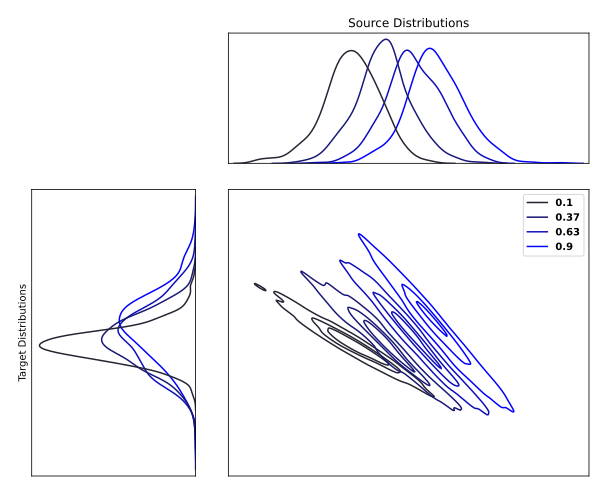
\includegraphics[scale=0.3]{chapter-3/images/plan_plot.pdf}
    \caption{The OT plans computed with the COT formulation (Eq.~\ref{eqn:impcot}) for the case of source and target as the conditional Gaussian distributions. For each value of the conditioned variable (shown as legends), we show the corresponding source, target and the obtained OT plan in a given color.}
    \label{fig:plan}
\end{figure}

\subsection{Cell Population Dynamics}
\paragraph{On Dataset.} We use the preprocessed dataset provided by \cite{cellot}. The dataset is publicly available for download using the following link \begin{verbatim}https://polybox.ethz.ch/index.php/s/RAykIMfDl0qCJaM.\end{verbatim} From this dataset, we extracted unperturbed cells and cells treated with \texttt{Givinostat}. This led to a total of 17,565 control cells and a total of 3,541 cells treated with \texttt{Givinostat}.  We take the same splits of data as in \cite{cellot}.

\paragraph{More on Evaluation.} Following \cite{Cuturi22}, we use \texttt{scanpy}'s \citep{Wolf2018} \texttt{rank\_genes\_groups} function for ranking and obtaining 50 marker genes for the drug, in this case \texttt{Givinostat}. The perturbed cells are grouped by drug, and the ranking is computed by keeping the unperturbed (i.e. control) cells as reference. We fix the architecture of our implicit model ($\psi$) as a 5-layer MLP and train it for 1000 epochs. Similar to \cite{Cuturi22}, we train on the 50-dimensional representation after applying PCA on the 1000-dimensional original representation. It is worth noting that training our MLP models is much stabler than the Partial Input Convex Neural Networks (PICNN) used in \cite{Cuturi22}, which needs carefully chosen initialization schemes. Following the evaluation scheme in \cite{Cuturi22}, we get back to the original 1000 dimensions, and then 50 marker genes are computed for the evaluation metrics.

Following \cite{Cuturi22}, we quantitatively evaluate our performance using the MMD distance and the $l_2$ distance between the perturbation signatures, $l_2$(PS) metric. Let $\mu$ be the set of observed unperturbed cell population, $\nu$ be the set of the observed perturbed cell population (of size $m_1$), and $\nu'$ be the set of predicted perturbed state of population $\mu$ (of size $m_2$). The perturbation signature $\textup{PS}(\nu, \mu)$ is then defined as 
$\frac{1}{m_1}\sum_{y_i\in\nu}y_i-\frac{1}{m_2}\sum_{y_i\in\mu}y_i'$. The $l_2$(PS) metric is the $l_2$ distance between $\textup{PS}(\nu, \mu)$ and $\textup{PS}(\hat{\nu}, \mu)$. 

\paragraph{More on Hyperparameters.}
Following \cite{Cuturi22}, we report evaluation based on MMD with RBF kernel averaged over the kernel widths: \{2, 1, 0.5, 0.1, 0.01, 0.005\}. Following the in-sample experiment done in \cite{Cuturi22}, we tune our hyperparameters on the training data split. Based on the scale of terms in the COT objective, we chose $\lambda_1=\lambda_2=\lambda$ from the set $\{400, 2000, 10000\}$ and found $\lambda=400$ to be the optimal choice. For the IMQ kernel, we chose the hyperparameter from the set $\{1, 10, 50, 100\}$ and found 100 to be the optimal choice. Since we model the transport plan and not the transport map, the following procedure is followed for inference. We generate one sample corresponding to each pair of (source sample, condition) through our implicit model, and measure the required metrics on the generated distributions. This procedure is repeated $n=50$ times, and the average metric is reported.

\begin{table}[t]
  \caption{In-sample setting: $l_2$ (PS) distances (lower is better) between predicted and ground truth distributions where the marker genes are computed at a per-dose level.}
  \label{sample-table-l2-perdose}
  \centering
  {
  \begin{tabular}{cccc}
    \toprule
        Dosage   & CellOT & CondOT & \cellcolor{green!10}{Proposed (COT)} \\  
        \midrule
        % CPA & 2.47$\pm$2.89 \\
        $10nM$ & 0.7164 & 0.4718 & \cellcolor{green!10}{\textbf{0.3682}} \\
        $100nM$ & 0.5198 & 0.3267 & \cellcolor{green!10}{\textbf{0.3051}}\\
        $1000nM$ & 0.7075 & 0.6982 & \cellcolor{green!10}{\textbf{0.3917}} \\
        $10000nM$ & 4.8131 & 0.3457 & \cellcolor{green!10}{\textbf{0.2488}}  \\
        %\textbf{Average} & 1.6892 & 0.4606 &  \textbf{0.3284}\\
        \bottomrule 
  \end{tabular}}
\end{table}

\begin{table}[t]
  \caption{In-sample setting: MMD distances (lower is better) between predicted and ground truth distributions where the marker genes are computed at a per-dose level.}
  \label{sample-table-mmd-perdose}
  \centering
  {
  \begin{tabular}{cccc}
    \toprule
        Dosage   & CellOT & CondOT & \cellcolor{green!10}{Proposed (COT)} \\  
        \midrule
        % CPA & 2.47$\pm$2.89 \\
        $10nM$ & 0.0089 & 0.0064 & \cellcolor{green!10}{\textbf{0.00549}} \\
        $100nM$ & 0.0069 & 0.0054 & \cellcolor{green!10}{\textbf{0.00494}}\\
        $1000nM$ & 0.0117 & 0.01038 & \cellcolor{green!10}{\textbf{0.00586}} \\
        $10000nM$ & 0.16940 & 0.01051 & \cellcolor{green!10}{\textbf{0.01011}}  \\
        % \textbf{Average} & 0.04922 & 0.00817 &  \textbf{0.00660}\\
        \bottomrule 
  \end{tabular}}
\end{table}


\paragraph{Additional Results.} In addition to the results reported in Tables \ref{sample-table-l2} and \ref{sample-table-mmd} where the marker genes are computed on a per-drug level, in Tables \ref{sample-table-l2-perdose} and \ref{sample-table-mmd-perdose}, we show results where marker genes are computed on a per-dosage level.
Further, we present results for the out-of-sample setting, i.e., the dosage levels we predict are not seen during training. In Tables \ref{oos-l2} and \ref{oos-mmd}, we show the results when marker genes are computed on a per-drug level and in Tables \ref{oos-l2-dose} and \ref{oos-mmd-dose}. we show the results when marker genes are computed on a per-dose level. In Figures \ref{fig:marginal} and \ref{fig:marginal-o}, we also show how closely the marginals of the proposed conditional optimal transport plan match the target distribution. The plots for COT correspond to the generated distribution having the median value for the metrics among all the (n=50) generated distributions. 
\begin{table}[t]
  \caption{Out-of-sample setting: $l_2$ (PS) distances (lower is better) between predicted and ground truth distributions where the marker genes are computed at a per-drug level.}
  \label{oos-l2}
  \centering
  {
  \begin{tabular}{cccc}
    \toprule
        Dosage   & CellOT & CondOT & Proposed (COT) \\  
        \midrule
        $10nM$ & 2.0889 & 0.3789 & \textbf{0.3376} \\
        $100nM$ & 2.0024 & 0.2169 & \textbf{0.1914}\\
        $1000nM$ & 1.2596 & \textbf{0.9928} & 1.002 \\
        $10000nM$ & \textbf{5.9701} & 34.9016 & 8.2417  \\
        \bottomrule 
  \end{tabular}}
\end{table}

\begin{table}[t]
  \caption{Out-of-sample setting: MMD distances (lower is better) between predicted and ground truth distributions where the marker genes are computed at a per-drug level.}
  \label{oos-mmd}
  \centering
  {
  \begin{tabular}{cccc}
    \toprule
        Dosage   & CellOT & CondOT & Proposed (COT) \\  
        \midrule
        $10nM$ & 0.0369 & \textbf{0.0065} & 0.0071 \\
        $100nM$ & 0.0342 & \textbf{0.0061}  & 0.0070\\
        $1000nM$ & 0.0215 & 0.0178 & \textbf{0.0151} \\
        $10000nM$ & \textbf{0.2304} & 0.3917 & 0.3591  \\
        % \textbf{Average} & 0.04922 & 0.00817 &  \textbf{0.00660}\\ .105525 .097075
        \bottomrule 
  \end{tabular}}
\end{table}

\begin{table}
  \caption{Out-of-sample setting: $l_2$ (PS) distances (lower is better) between predicted and ground truth distributions where the marker genes are computed at a per-dose level.}
  \label{oos-l2-dose}
  \centering
  {
  \begin{tabular}{cccc}
    \toprule
        Dosage   & CellOT & CondOT & Proposed (COT) \\  
        \midrule
        $10nM$ & 1.2130 & 0.4718 & \textbf{0.3950} \\
        $100nM$ & 0.8561 & 0.2846 & \textbf{0.2522}\\
        $1000nM$ & \textbf{0.9707} & 0.9954 & 1.0775 \\
        $10000nM$ & \textbf{5.8737} & 33.5211 & 7.1487  \\
        \bottomrule 
  \end{tabular}}
\end{table}

\begin{table}
  \caption{Out-of-sample setting: MMD distances (lower is better) between predicted and ground truth distributions where the marker genes are computed at a per-dose level.}
  \label{oos-mmd-dose}
  \centering
  {
  \begin{tabular}{cccc}
    \toprule
        Dosage   & CellOT & CondOT & Proposed (COT) \\  
        \midrule
        $10nM$ & 0.01648 & 0.00641 & \textbf{0.00638} \\
        $100nM$ & 0.01133 & 0.006325  & \textbf{0.00571}\\
        $1000nM$ & 0.01607 & 0.01496 & \textbf{0.01462} \\
        $10000nM$ & \textbf{0.24234} & 0.41845 & 0.34246  \\
        % \textbf{Average} & 0.04922 & 0.00817 &  \textbf{0.00660}\\
        \bottomrule 
  \end{tabular}}
\end{table}

% \begin{figure}[t]
%     \centering
%     \includegraphics[width=0.3\textwidth]{chapter-3/images/ENSG00000165092.12_insample.pdf}
%     \includegraphics[width=0.3\textwidth]{chapter-3/images/ENSG00000175175.5_insample.pdf}
%     \includegraphics[width=0.3\textwidth]{chapter-3/images/ENSG00000173727.12_insample.pdf}
%     \caption{Marginals for selected genes `ENSG00000165092.12', `ENSG00000175175.5', `ENSG00000173727.12',  where the dosage is 100nM, in the in-sample setting.}
%     \label{fig:marginal}
% \end{figure}

\begin{figure}[t]
\centering
\begin{subfigure}{.4\textwidth}
    \centering
    \includegraphics[width=\textwidth]{chapter-3/images/C41.pdf}  
    \caption{For gene `ENSG00000165092.12'}
\end{subfigure}
\begin{subfigure}{.4\textwidth}
    \centering
    \includegraphics[width=\linewidth]{chapter-3/images/C42.pdf}  
    \caption{For gene `ENSG00000175175.5'}
    \label{fig:marginal}
\end{subfigure}
\caption{Marginal densities for selected genes where the dosage is 100nM, in the in-sample setting. The proposed COT plan's marginal densities resemble the target densities well.}
\end{figure}

% \begin{figure}[t]
%     \centering
%     \includegraphics[width=0.3\textwidth]{chapter-3/images/ENSG00000165092.12_outsample.pdf}
%     \includegraphics[width=0.3\textwidth]{chapter-3/images/ENSG00000175175.5_outsample.pdf}
%     \includegraphics[width=0.3\textwidth]{chapter-3/images/ENSG00000173727.12_outsample.pdf}
%     \caption{Marginals for selected genes `ENSG00000165092.12', `ENSG00000175175.5', `ENSG00000173727.12',  where the dosage is 100nM, in the out-sample setting.}
%     \label{fig:marginal-o}
% \end{figure}

\begin{figure}[t]
\centering
\begin{subfigure}{.4\textwidth}
    \centering
    \includegraphics[width=\textwidth]{chapter-3/images/C51.pdf}  
    \caption{For gene `ENSG00000165092.12'}
\end{subfigure}
\begin{subfigure}{.4\textwidth}
    \centering
    \includegraphics[width=\linewidth]{chapter-3/images/C52.pdf}  
    \caption{For gene `ENSG00000175175.5'}
    \label{fig:marginal-o}
\end{subfigure}
\caption{Marginal densities for selected genes where the dosage is 100nM, in the out-sample setting. The proposed COT plan's marginal densities resemble the target densities well.}
\end{figure}


% In Table \ref{table:time-exp}, we also show the per-epoch computation time taken (on an RTX 4090 GPU) by the COT loss as a function of the size of the minibatch, which shows the computational efficiency of the COT loss.

% \begin{table}[t]
%   \caption{Time (in s) for COT loss \ref{eqn:expexpcot} computation shown for increasing minibatch size. The computation time reported is based on 3 independent runs on the CIFAR-10 dataset.}
%   \label{table:time-exp}
%   \centering
%   \begin{tabular}{ccccc}
%     \toprule
%            & 16 & 64 & 512 & 1024 \\  
%         \midrule
%         Time (s) & 0.229$\pm$0.0013 & 0.229$\pm$0.0006 & 0.227$\pm$0.0004 & 0.225$\pm$0.0021 \\
%         \bottomrule 
%   \end{tabular}
% \end{table}
\begin{figure}[ht!]
    \centering
    \includegraphics[width=\columnwidth]{chapter-3/images/prompt-prop.pdf}
    \caption{The leftmost is an image from the EuroSAT satellite dataset followed by visualization maps corresponding to each of the 4 prompts learnt (using COT loss \ref{cot-prompt}). We can see that the 4 prompts diversely capture different visual features of the image.}
    \label{fig:prompt-prop}
\end{figure}
\subsection{Prompt Learning}
Let $\mathbf{F}=\{\mathbf{f}_m|_{m=1}^M\}$ denote the set of visual features for a given image and $\mathbf{G}_r=\{\mathbf{g}_n|_{n=1}^N\}$ denote the set of textual prompt features for class $r$. PLOT \citep{chen2023plot} learns the prompt features by performing an alternate optimization where the inner optimization solves an OT problem between the empirical measure over image features (49) and that over the prompt features (4). We denote the OT distance between the visual features of image $\mathbf{x}$ and the textual prompt features of class $r$ by $d_{OT}(\mathbf{x}, r)$. Then the probability of assigning the image $\mathbf{x}$ to class $r$ is computed as
$
    p(y=r|\mathbf{x}) = \frac{\exp{\left((1-d_{OT}(\mathbf{x}, r)/\tau)\right)}}{\sum_{r=1}^T\exp{\left((1-d_{OT}(\mathbf{x}, r)/\tau)\right)}},
$ where $T$ denotes the total no. of classes and $\tau$ is the temperature of softmax. These prediction probabilities are then used in the cross-entropy loss for the outer optimization.

Following \cite{chen2023plot} and \cite{coop}, we choose the last training epoch model. The PLOT baseline empirically found 4 to be the optimal number of prompt features. We follow the same for our experiment. We also keep the neural network architecture and hyperparameters the same as in PLOT. For our experiment, we choose $\lambda_1=\lambda_2=\lambda$, kernel type and the kernel hyperparameter used in COT. We choose the featurizer in Fig.~\ref{prompt-diag} as the same image encoder used for getting the visual features. We use a 3-layer MLP architecture for $\psi_r$ in Eq. \ref{cot-prompt}. Fig. \ref{fig:prompt-prop} shows attention maps corresponding to each of the prompts learnt by COT. We choose $\lambda$ from \{1, 10, 100\}, kernel type from {$k(x, y) = \exp{\frac{-\|x-y\|^2}{2\sigma^2}}$ (referred as RBF), $k(x, y)=(\sigma^2+\|x-y\|^2)^{-0.5}$ (referred as IMQ), $k(x, y) = \left(\frac{1+\|x-y\|^2}{\sigma^2} \right)^{-0.5}$(referred as IMQ2)}, kernel hyperparameter ($\sigma^2$) from \{median, 0.01, 0.1, 1, 10, 100\}. The chosen hyperparameters, ($\lambda$, kernel type, kernel hyperparameter), for the increasing number of shots (1 to 8), are (100, RBF, 10), (100, IMQ2, 1), (10, IMQ, 1), (1, IMQ, 0.01). Table \ref{tbl:prompt-abl} presents an ablation study.

\begin{figure}[ht!]
    \centering
    \includegraphics[width=\columnwidth]{chapter-3/images/prompt-ablation.pdf}
    \caption{Ablation study for the prompt learning experiment $\mathcal{F}=1$. For different kernel types: (a) RBF kernel $k(x, y)=\exp{\left(\frac{-\|x-y\|^2}{2\sigma^2}\right)}$ (b) IMQ kernel $k(x, y)=\left(\sigma^2+\|x-y\|^2\right)^{-0.5}$ (c) IMQ kernel $k(x, y) = \left(\frac{1+\|x-y\|^2}{\sigma^2} \right)^{-0.5}$, we show the average accuracy for different kernel hyperparameters (shown on the x-axis) and different lambda values.}
    \label{tbl:prompt-abl}
\end{figure}





%%
\resumetoc